\section{Winoground}

We perform various experiments on Winoground. Appart from image-text matching \ref{image_text_matching}, we perform more experiments to gain more insight about the dataset and the tested models.

\subsection{Image-Text Matching} \label{image_text_matching}

This is the original Winoground task, given two captions and two images the aim is to match them correctly.

\subsection{Text-to-Image Generation} \label{text_to_image_generation}

We used Stable Diffusion to generate images 9 images for each Winoground caption. This results in a total of $800*9=7200$ images. See \cref{fig:stable-diffusion-examples}, \cref{fig:stable-diffusion-examples-linguistic} and \cref{fig:stable-diffusion-examples-visual} for a few examples of generated images.

We used Label Studio to annotate images generated by Stable Diffusion. As annotating all the images would take a very long time, we choose to annotate a subset of examples, and only one image per caption.

In each annotation there are two captions from Winoground and two images generated with Stable Diffusion. Each image is created from one caption but the order of the images is random. The annotators have to choose which text corresponds to each image: the first caption, the second caption, both or none. An screenshot of the annotation interface can be seen in...

There were 5 annotators in total and each one annotated 50 examples, for a total of 250 annotated examples. There are 400 examples in total, so we decided that it is a big enough subset.

The general conclusion is that Stable Diffusion is not good at this task. Most of the images do not match any of the captions. There are a few images that match both captions. The remaining images match one caption or the other, but there are many that match the incorrect caption. If we take into account image pairs, there are only a few correct ones.

\begin{figure}
\centering
    \begin{minipage}[t]{.30\textwidth}
        \begin{subfigure}[t]{\textwidth}
        \centering
        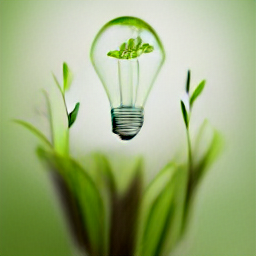
\includegraphics[height=4cm]{ex_155_cap_0_img_0.png}
        \caption{[some plants] surrounding [a lightbulb]}
        \end{subfigure}\\
        \begin{subfigure}[t]{\textwidth}
        \centering
        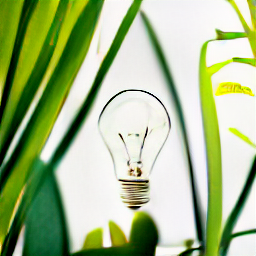
\includegraphics[height=4cm]{ex_155_cap_1_img_0.png}
        \caption{[a lightbulb] surrounding [some plants]}
        \end{subfigure}%
        \caption{\textit{Object}}
    \end{minipage}
    \hfill
    \begin{minipage}[t]{.30\textwidth}
        \begin{subfigure}[t]{\textwidth}
        \centering
        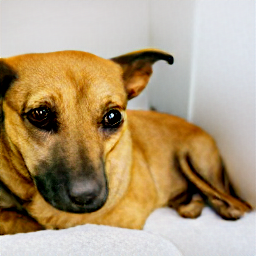
\includegraphics[height=4cm]{ex_29_cap_0_img_0.png}
        \caption{a [brown] dog is on a [white] couch}
        \end{subfigure}\\
        \vspace{9pt}
        \begin{subfigure}[t]{\textwidth}
        \centering
        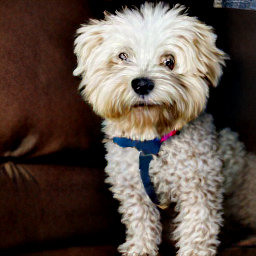
\includegraphics[height=4cm]{ex_29_cap_1_img_0.png}
        \caption{a [white] dog is on a [brown] couch}
        \end{subfigure}%    
        \caption*{\textit{Relation}}
    \end{minipage}
    \hfill
    \begin{minipage}[t]{.30\textwidth}
        \begin{subfigure}[t]{\textwidth}
        \centering
        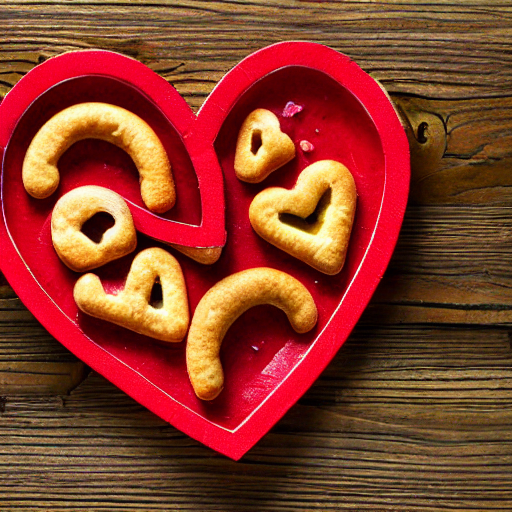
\includegraphics[height=4cm]{ex_118_cap_1_img_0.png}
        \caption{[circular] food on [heart-shaped] wood}
        \end{subfigure}\\
        \begin{subfigure}[t]{\textwidth}
        \centering
        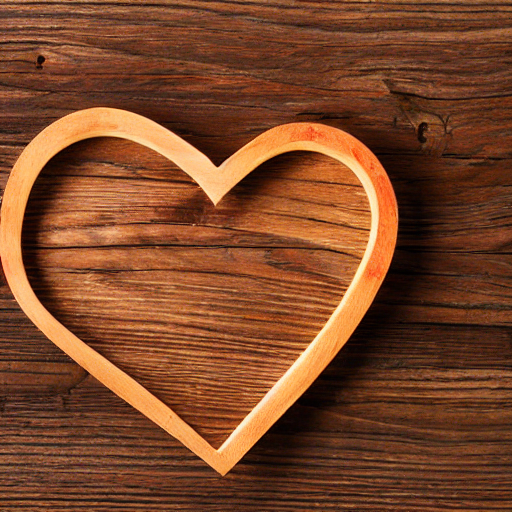
\includegraphics[height=4cm]{ex_118_cap_0_img_0.png}
        \caption{[heart-shaped] food on [circular] wood}
        \end{subfigure}%
        \caption*{\textit{Relation}}
    \end{minipage}%
    \caption[]{Stable Diffusion examples for the swap-dependent linguistic tags \textit{Object}, \textit{Relation} and \textit{Relation} from left to right. The linguistic examples are additionally tagged with 1 main predicate.}
    \label{fig:stable-diffusion-examples}
\end{figure}

\begin{figure}
\centering
    \begin{minipage}[t]{.30\textwidth}
        \begin{subfigure}[t]{\textwidth}
        \centering
        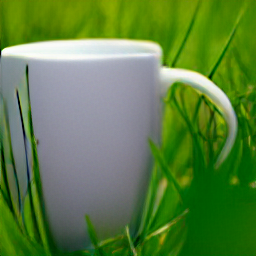
\includegraphics[height=4cm]{ex_14_cap_0_img_0.png}
        \caption{there is [a mug] in [some grass]}
        \end{subfigure}\\
        \begin{subfigure}[t]{\textwidth}
        \centering
        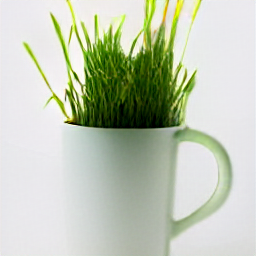
\includegraphics[height=4cm]{ex_14_cap_1_img_0.png}
        \caption{there is [some grass] in [a mug]}
        \end{subfigure}%    
        \caption*{\textit{Object}}
    \end{minipage}
    \hfill
    \begin{minipage}[t]{.30\textwidth}
        \begin{subfigure}[t]{\textwidth}
        \centering
        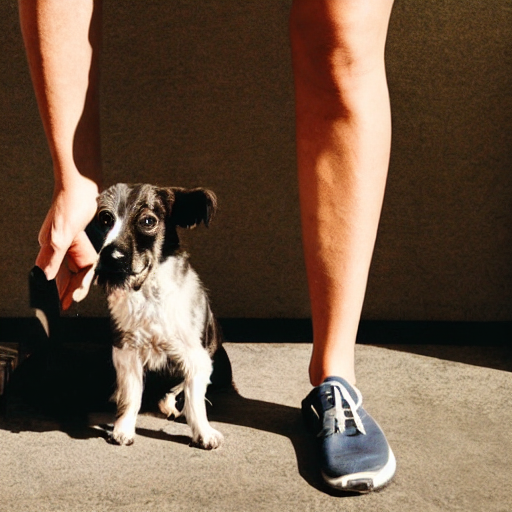
\includegraphics[height=4cm]{ex_21_cap_0_img_0.png}
        \caption{a person [sits] and a dog [stands]}
        \end{subfigure}\\
        \begin{subfigure}[t]{\textwidth}
        \centering
        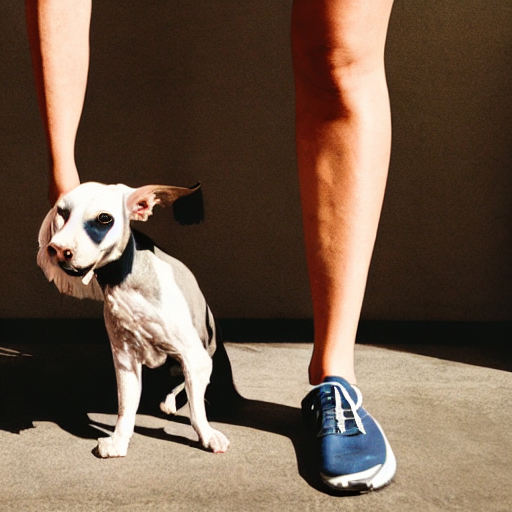
\includegraphics[height=4cm]{ex_21_cap_1_img_0.png}
        \caption{a person [stands] and a dog [sits]}
        \end{subfigure}%    
        \caption*{\textit{Relation}}
    \end{minipage}
    \hfill
    \begin{minipage}[t]{.30\textwidth}
        \begin{subfigure}[t]{\textwidth}
        \centering
        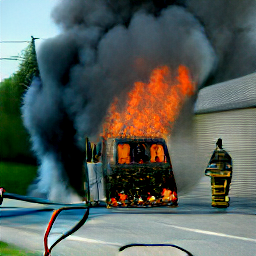
\includegraphics[height=4cm]{ex_72_cap_1_img_0.png}
        \caption{it's a [truck] [fire]}
        \end{subfigure}\\
        \begin{subfigure}[t]{\textwidth}
        \centering
        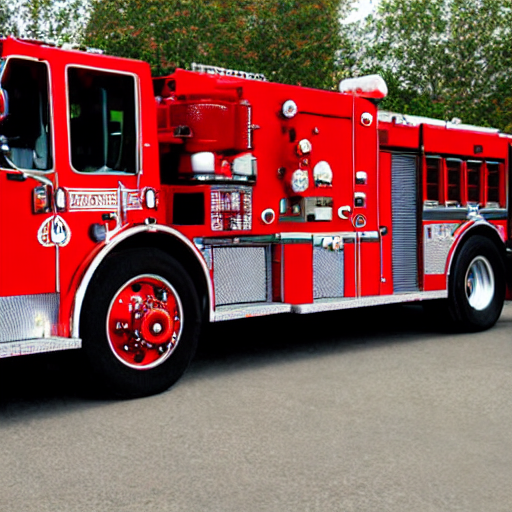
\includegraphics[height=4cm]{ex_72_cap_0_img_0.png}
        \caption{it's a [fire] [truck]}
        \end{subfigure}%
        \caption*{\textit{Both}}
    \end{minipage}%
    \caption[]{Stable Diffusion examples for the swap-dependent linguistic tags \textit{Object}, \textit{Relation} and \textit{Both} from left to right. The linguistic examples are additionally tagged with 2, 1, and 1 main predicates from left to right.}
    \label{fig:stable-diffusion-examples-linguistic}
\end{figure}

\begin{figure}
\centering
    \begin{minipage}{.30\textwidth}
        \begin{subfigure}{\textwidth}
        \centering
        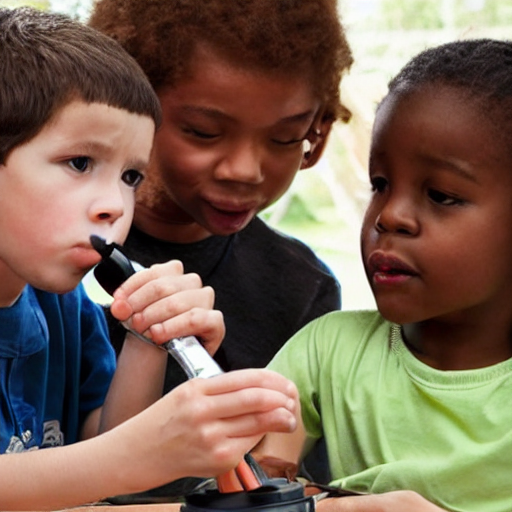
\includegraphics[height=4cm]{ex_75_cap_0_img_0.png}
        \caption{the kid [with the magnifying glass] looks at them []}
        \end{subfigure}\\
        \begin{subfigure}{\textwidth}
        \centering
        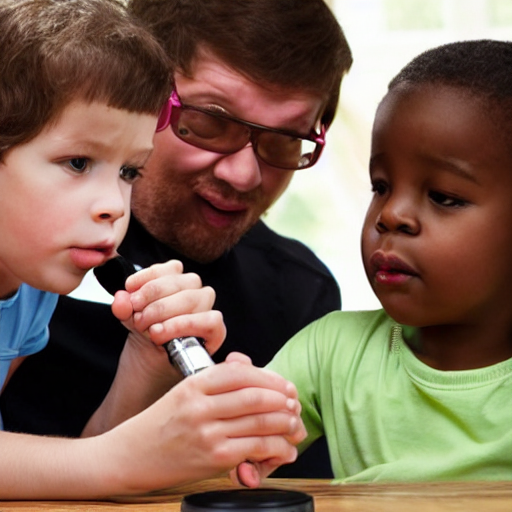
\includegraphics[height=4cm]{ex_75_cap_1_img_0.png}
        \caption{the kid [] looks at them [with the magnifying glass]}
        \end{subfigure}%    
        \caption*{\textit{Pragmatics}}
    \end{minipage}
    \hfill
    \begin{minipage}{.30\textwidth}
        \begin{subfigure}{\textwidth}
        \centering
        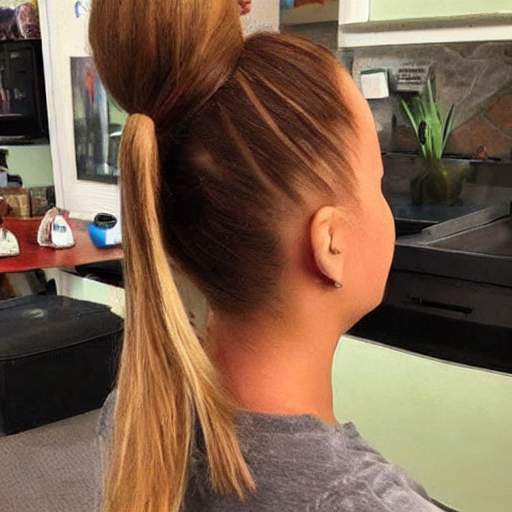
\includegraphics[height=4cm]{ex_27_cap_0_img_0.png}
        \caption{the person with the ponytail [packs] stuff and other [buys] it}
        \end{subfigure}\\
        \begin{subfigure}{\textwidth}
        \centering
        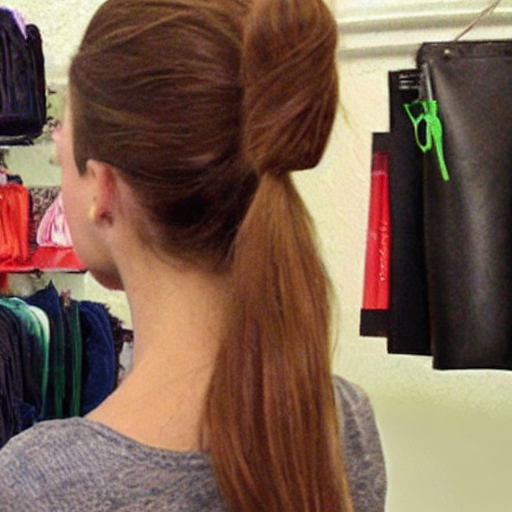
\includegraphics[height=4cm]{ex_27_cap_1_img_0.png}
        \caption{the person with the ponytail [buys] stuff and other [packs] it}
        \end{subfigure}%    
        \caption*{\textit{Series}}
    \end{minipage}
    \hfill
    \begin{minipage}{.30\textwidth}
        \begin{subfigure}{\textwidth}
        \centering
        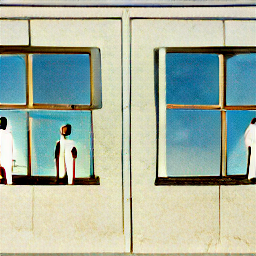
\includegraphics[height=4cm]{ex_61_cap_0_img_0.png}
        \caption{there are [three] people and [two] windows}
        \end{subfigure}\\
        \begin{subfigure}{\textwidth}
        \centering
        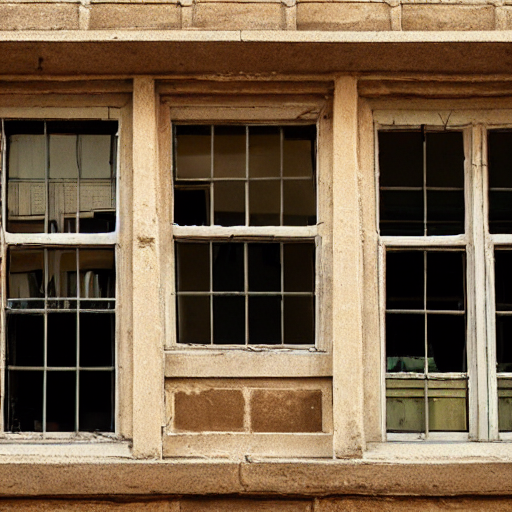
\includegraphics[height=4cm]{ex_61_cap_1_img_0.png}
        \caption{there are [two] people and [three] windows}
        \end{subfigure}%    
        \caption*{\textit{Symbolic}}
    \end{minipage}
    \caption[]{Stable Diffusion examples for the swap-dependent visual tags \textit{Pragmatics}, \textit{Series} and \textit{Symbolic} from left to right. The visual examples are additionally tagged with the \textit{Relation} tag, and 1, 2, and 1 main predicates from left to right.}
    \label{fig:stable-diffusion-examples-visual}
\end{figure}

\subsection{Image Captioning} \label{image_captioning}

We used OFA \cite{wang2022unifying} and BLIP \cite{li2022blip} models of different sizes to generate captions for all Winoground images. We chose these models because they are SOTA in image captioning and we also use them in other evaluations. Our intention was to compare them with the real captions. We calculated BLEU scores for all models and we found out that they are very low. This indicates that the captions generated by these models are very far from the real captions. 

One reason for this could be that the real Winoground captions are not typical captions. They are hand-crafted so that they contain the same words in a different order, and that conditions the captions. Another reason could be that these models are not good at describing these types of images that require compositional reasoning. As these models are not very good at matching Winoground images with captions.

Analysing the captions manually would be necessary to know how good they really are. If these captions are good enough they could also be used to improve the results of the models by incorporating them in the evaluation process. They could provide extra information about the images to the models, that is not included in the original captions.

\subsection{Image Retrieval} \label{image_retrieval}

We used CLIP retrieval\footnote{\url{https://github.com/rom1504/clip-retrieval}} to retrieve images from LAION-5B dataset. We used Winoground captions and images to get similar images. For each caption and image, we compute its embeddings using CLIP ViT-L-14. Then the system uses a KNN algorithm to retrieve images that have similar embeddings. We can also compute the mean of caption and image embeddings to retrieve images that match both the image and the caption.

The system also has an aesthetic score that can be used to retrieve better looking images. It can also remove duplicate images and images that contain unsafe content and violence.

This system can be used to increase the size of our dataset. We can retrieve many similar images. The number of retrieved images and the similarity score can also be used as a measure of how common an image is. If there are very few similar images in the dataset, that means that the image is uncommon.